% Author: Savin Ivan xsavini00
% Author: Turar Nurdaulet xturarn00
% Author: Krasovskyi Oleh xkrasoo00 
% Author: Popov Albert xpopov10 


\documentclass[a4paper, 11pt]{article}


\usepackage[english]{babel}
\usepackage[utf8]{inputenc}
\usepackage[left=2cm, top=3cm, text={17cm, 24cm}]{geometry}
\usepackage[unicode,pdftitle={Překladač jazyka IFJ24},hidelinks]{hyperref}
\usepackage{times}
\usepackage{forest} % В преамбуле документа подключите пакет forest
\usepackage{verbatim}
\usepackage{enumitem}
\usepackage{graphicx} % vkládání obrázků
\usepackage{longtable}
\usepackage{amsmath}
\hypersetup{
	colorlinks = true,
	hypertexnames = false,
	citecolor = red
}


\newcommand{\RNum}[1]{\uppercase\expandafter{\romannumeral #1\relax}} % makro na sázení římských čísel


\begin{document}


	%%%%%%%%%%%%%%%%%%%%%%%%%%%%%%%% Titulní stránka %%%%%%%%%%%%%%%%%%%%%%%%%%%%%%%%
	\begin{titlepage}
		\begin{center}
			
\includegraphics[width=0.77\linewidth]{FIT_logo.png} \\

			\vspace{\stretch{0.382}}

			\Huge{Project documentation} \\
			\LARGE{\textbf{Implementace překladače imperativního jazyka IFJ24}} \\
			\Large{Tým xpopov10, varianta vv-BVS}
			\vspace{\stretch{0.618}}
		\end{center}

		\begin{minipage}{0.4 \textwidth}
			{\Large \today}
		\end{minipage}
		\hfill
		\begin{minipage}[r]{0.6 \textwidth}
			\Large
			\begin{tabular}{l l l}
				\textbf{Popov Albert} & \textbf{(xpopov10)} & \quad 25\,\% \\
				Krasovskyi Oleh & (xkrasoo00) & \quad 25\,\% \\
				Savin Ivan & (xsavini00) & \quad 25\,\% \\
				Turar Nurdaulet & (xturarn00) & \quad 25\,\% \\
			\end{tabular}
		\end{minipage}
	\end{titlepage}



	%%%%%%%%%%%%%%%%%%%%%%%%%%%%%%%% Introduction %%%%%%%%%%%%%%%%%%%%%%%%%%%%%%%%
	\pagenumbering{arabic}
	\setcounter{page}{1}

	\section{Introduction}

	The goal of the project was to create a C program that reads source code written in the IFJ24 source language,
    which is a simplified subset of the imperative programming language Zig 0.13, and translates it into the target language IFJcode24 (intermediate code).
    
    The program is a console application that reads the source program from standard input and generates
    the resulting intermediate code to the standard output or, in the event of an error, returns the corresponding error code.



    %%%%%%%%%%%%%%%%%%%%%%%%%%%%%%%% Work in the team %%%%%%%%%%%%%%%%%%%%%%%%%%%%%%%%
	\section{Work in the team}

	\subsection{How the team works}

    At the beginning of the project, we divided the task into 4 main blocks and acted according to the interaction of the codes. If someone's work seemed less important, that person helped others or wrote tests.
	\subsubsection{Version control system}

	We used the Git versioning system to manage the project files. As a remote repository we used \mbox{GitHub}.

	Git allowed us to work on multiple tasks on a project at the same time in so-called branches. Most of the tasks were first prepared
	into a branch, and only after testing and approving the modifications by other team members did we incorporate them into the main
	development branch.

	\subsubsection{Communication}

	Communication was in general conversation or private messages.

	Towards the end of the project, we met to demonstrate how our program blocks worked, in order to find errors and increase the understanding of the project to the other participants.


	\subsection{Distribution of work among team members}

	We divided the work on the project evenly with regard to its complexity and time demands.
	So everyone got a percentage rating of 25\,\%.
	The table summarizes the distribution of the team's work among the individual members.
	\bigskip
	\begin{table}[ht]
		\centering
		\begin{tabular}{| l | l |}
			\hline
			Team Member & Assigned Work \\ \hline
			\textbf{Popov Albert} & \begin{tabular}{l} team management, testing, syntactic analysis  \end{tabular} \\
			Krasovskyi Oleg & \begin{tabular}{l} semantic analysis, testing \end{tabular} \\
			Savin Ivan & \begin{tabular}{l}lexical analysis, documentation, testing \end{tabular} \\
			Turar Nurdaulet & \begin{tabular}{l} target code generation, work organization, testing, project structure\end{tabular} \\ \hline
		\end{tabular}
		\caption{Distribute the work of the team among the individual members}
		\label{table:rozdeleni_prace}
	\end{table}


	%%%%%%%%%%%%%%%%%%%%%%%%%%%%%%%% Návrh a implementace %%%%%%%%%%%%%%%%%%%%%%%%%%%%%%%%
	\section{Design and implementation}

	The project is composed of several parts implemented by us, which are presented in this chapter.
	It also shows how the different subparts work together.

    \subsection{Compiler structure}
    The compiler consists of the following modules:\\
    \textbf{Lexical analyzer (lexer):} Converts source code to tokens\\
    \textbf{Parser:} It analyzes tokens using syntactic and semantic rules and then builds an abstract syntax tree (AST).\\
    \textbf{Code Generator:} Generates target code from AST.
   
    The finite automaton diagram for the lexer and the LL table will be attached in separate attachments.

	\subsection{Lexical Analysis}

        The first stage of the compiler is lexical analysis. Initially, we assumed that a separator symbol would exist between all tokens, allowing the source code to be divided into discrete blocks. Each block could then be easily converted into corresponding tokens. However, this approach was abandoned due to the need to implement numerous exceptions in certain cases, which made the lexer harder to extend and reduced code readability.
        
        The new version of the lexical analyzer employs a deterministic finite automaton (DFA). The main function, \texttt{run\_lexer()}, reads the input code and starts the automaton in its initial state. It identifies the first non-empty character and transitions the automaton to the corresponding state. After processing that state, the control returns to \texttt{run\_lexer()}, which continues reading until the end of the file.
    
        \textbf{Processing Identifiers}
    
        For identifiers, allowed characters are read sequentially. Once the sequence is fully read, the lexer determines whether it matches a keyword or should be classified as an identifier. This approach allows keywords to be correctly identified and associated tokens to be created.
    
        \textbf{Processing Numbers}
    
        For numerical tokens, digits, decimal points, and the characters \texttt{e/E} are read in sequence. If the input forms a valid number, the lexer generates an \texttt{f64} or \texttt{i32} token based on the data provided.
        
        \textbf{Finite State Machine Design}
        
        The entire lexical analyzer is implemented as a deterministic finite automaton based on a predefined state diagram (included in the appendix). This diagram defines the states and transitions, ensuring the lexer is easier to maintain and extend when required.
        
        By utilizing a structured DFA approach, the lexer achieves a balance between functionality and simplicity, making it a reliable component of the compiler pipeline.


	\subsection{Syntactic Analysis}

        The syntactic analyzer, or parser, ensures that the input source code adheres to the defined grammar of the programming language. It processes the sequence of tokens produced by the lexical analyzer and organizes them into an Abstract Syntax Tree (AST), which represents the hierarchical structure of the program.
        
        \textbf{How it works}
        
        \textbf{Input:}  
        The parser takes a sequence of tokens from the lexical analyzer. Each token consists of its type and optionally its attributes (e.g., literal values or identifier names).
        
        \textbf{Parsing Strategy:}  
        The parser uses a recursive descent parsing approach. Each grammatical rule is implemented as a specific function that matches tokens and recursively processes nested structures.
        
        \textbf{Abstract Syntax Tree (AST):}  
        The parser constructs an AST for syntactically valid input. The AST represents program constructs such as expressions, statements, and function definitions in a hierarchical form. For example, an expression like \texttt{a + b * c} is represented as a tree with \texttt{+} as the root, \texttt{a} as the left child, and a subtree for \texttt{b * c} as the right child.
        
        \textbf{Error Handling:}  
        The parser reports syntax errors if a token does not match the expected grammar rule. For example, if a semicolon is missing, the parser will report an error and gracefully terminate with a message indicating the expected token and its position.
        
        \subsubsection*{Workflow}
        
        \textbf{Initialization:}  
        Parsing begins with the \texttt{parseProgram} function, which processes the overall program structure. It first validates the prologue and then processes all function definitions.
        
        \textbf{Recursive Descent Parsing:}  
        Each grammar rule is implemented as a function (e.g., \texttt{parseExpression}, \texttt{parseStatement}). These functions match tokens and recursively call other functions to process nested constructs.
        
        \textbf{Token Matching:}  
        The \texttt{match} function ensures the current token matches the expected type. If not, a syntax error is raised.
        
        \textbf{AST Construction:}  
        For valid input, the parser creates AST nodes using helper functions like \texttt{createASTNode} and \texttt{createBinaryASTNode}. These nodes capture the syntactic structure of constructs such as expressions, statements, and function definitions.
        
        \textbf{Completion:}  
        After processing all tokens, the parser finalizes the AST, which is then passed to the semantic analyzer for further validation.
        
        
        \subsubsection*{Example Workflow}
        
        \begin{verbatim}
        const ifj = @import("ifj24.zig");
        
        pub fn main() void {
            var x: i32 = 5; 
            x = x + 1;
            return;
        }
        \end{verbatim}
        
        The parser verifies the validity of the prologue: \texttt{const ifj = @import("ifj24.zig");}.  
        It analyzes the function definition \texttt{pub fn main() void}.  
        Inside \texttt{main}, it analyzes:  
        - Variable declaration: \texttt{var x: i32 = 5}.  
        - Assignment: \texttt{x = x + 1}.  
        - Return statement: \texttt{return}.  
        
        The resulting AST has the following structure:  
        
        \begin{verbatim}
        Program
        ├── Prolog
        └── FunctionDef (main)
            ├── Parameters: None
            ├── ReturnType: void
            └── StatementList
                ├── VarDeclaration (x: i32 = 5)
                ├── Assignment (x = x + 1)
                └── Return
        \end{verbatim}
        
        The AST is then passed to the semantic analyzer.

	\subsection{Semantic analysis}

    	Semantic analysis
    

	\subsection{Target code generation}

	\begin{itemize}
    \item \texttt{target\_gen.h}: An entry point to the target code generation.
    \item \texttt{target\_func\_context.h}: Used to store all instructions to be used within a function context. Variable definitions (DEFVAR Instructions) are stored separately and outputted first. Then, other instructions are outputted. It's done so that each variable is defined only once within a scope. If its done more often, a program will crash. It can happen if a variable declaration is done within a loop.
    \item \texttt{id\_indexer.h}: Used to add a unique index for labels and each function scope, in order to avoid label/variable name collisions.
    \item \texttt{instructions.h}: Module that encapsulates the target code's instructions construction.
    
    \end{itemize}

	%%%%%%%%%%%%%%%%%%%%%%%%%%%%%%%% Conclusion %%%%%%%%%%%%%%%%%%%%%%%%%%%%%%%%
	\section{Conclusion}

	The project initially surprised us a bit with its scope and complexity. Over time, until we had enough
	knowledge about compiler development from the IFJ lectures, we started to tackle the project.

	We had our team assembled very early on, and we had already agreed on the communication channels in advance,
	face-to-face meetings and the use of the versioning system, so we didn't have any
	and we worked very well together.

	We started working on the project a bit late, so we didn't have time to spare, but in the end
	we got everything done. We worked on the different parts of the project mostly individually using
	knowledge from lectures or materials for IFJ and IAL courses.

	During the development, we encountered minor problems related to ambiguities in the assignment, but
	these have been resolved through the project forum. The correctness of the solution was verified by automatic
	tests and ~test submissions, which allowed us to further fine-tune the project.

	Overall, this project has given us a lot of knowledge about how compilers work, practically
	clarified the subject matter covered in the IFJ and ~IAL courses, and~brought us experience with~projects of this magnitude.

	%%%%%%%%%%%%%%%%%%%%%%%%%%%%%%%% Attachments %%%%%%%%%%%%%%%%%%%%%%%%%%%%%%%%
	\clearpage
	\appendix


	%\section{Diagram konečného automatu specifikující lexikální analyzátor}
	%\begin{figure}[!ht]
	%	\centering
	%	\vspace{-1.2cm}
	%	\includegraphics[width=0.95\linewidth]{inc/FA_graph.pdf}
	%	\caption{Diagram konečného automatu specifikující lexikální analyzátor}
	%	\label{figure:fa_graph}
	%\end{figure}

	\begin{table}[!ht]
        \section{Grammar}
		\centering
		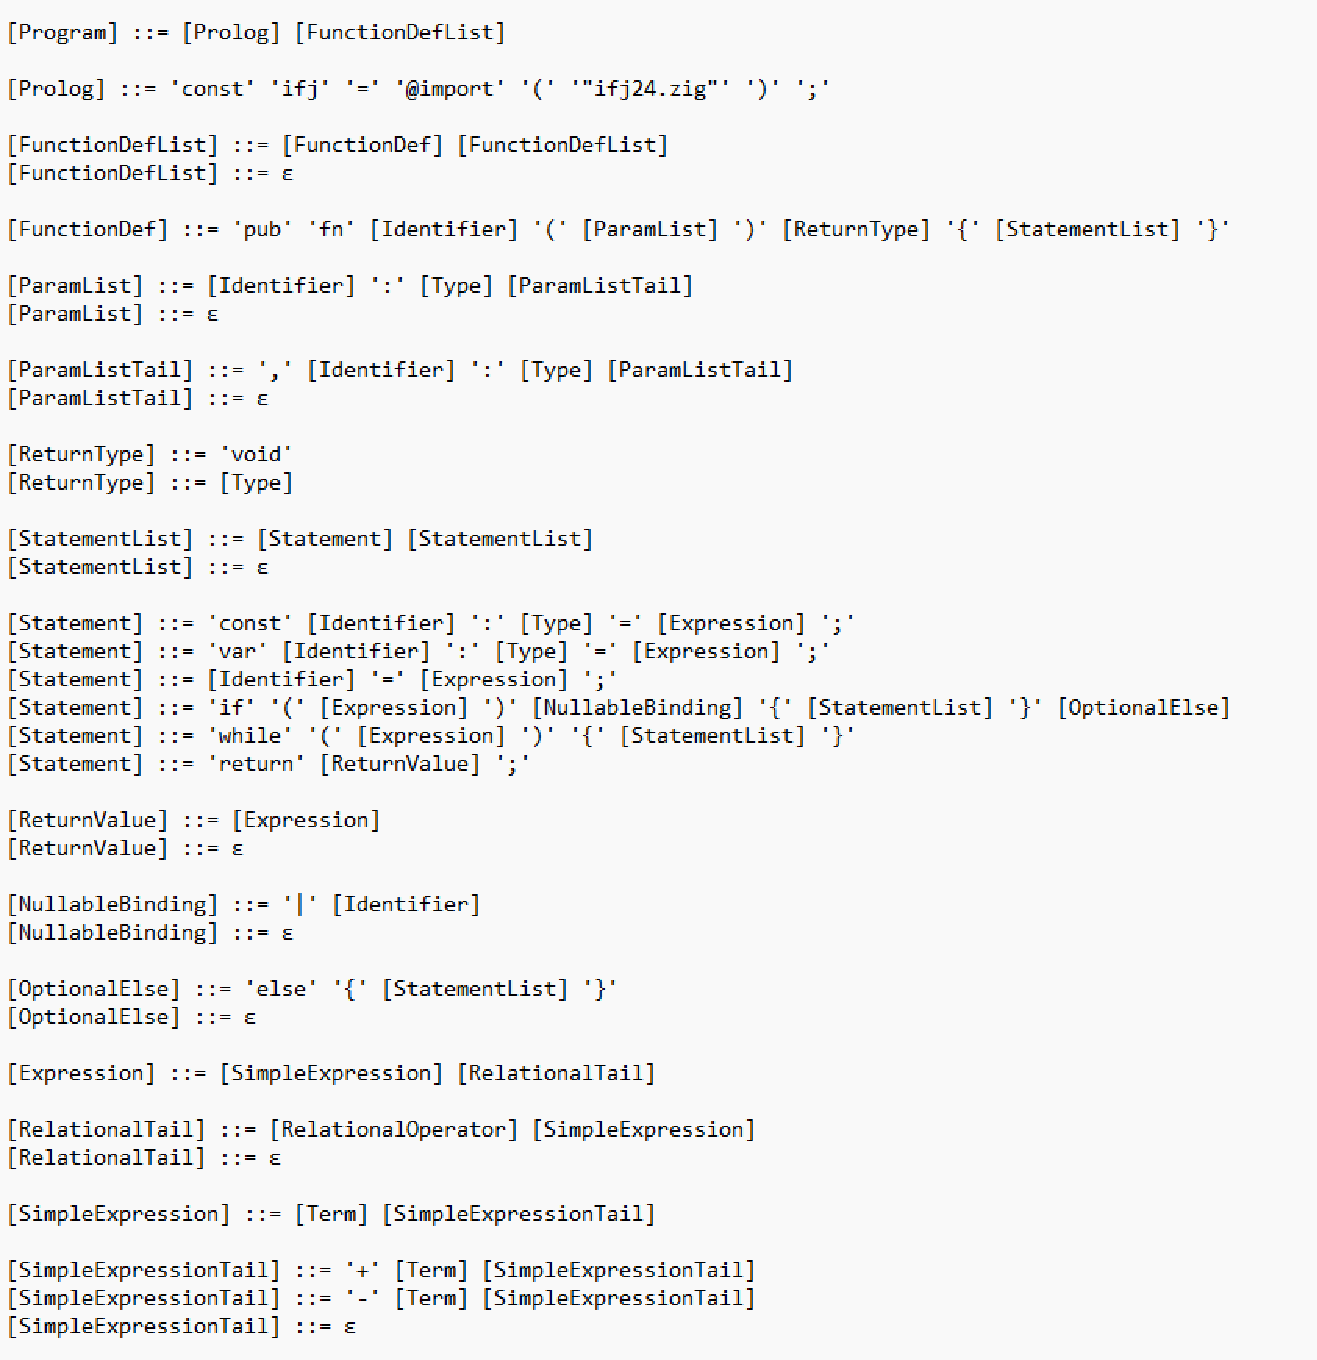
\includegraphics[width=1\linewidth]{Grammar1.pdf}
		\caption{Grammar 1}
		\label{table:png2pdf (1).pdf}
	\end{table}

    
	\begin{table}[!ht]
        \section{Grammar2}
		\centering
		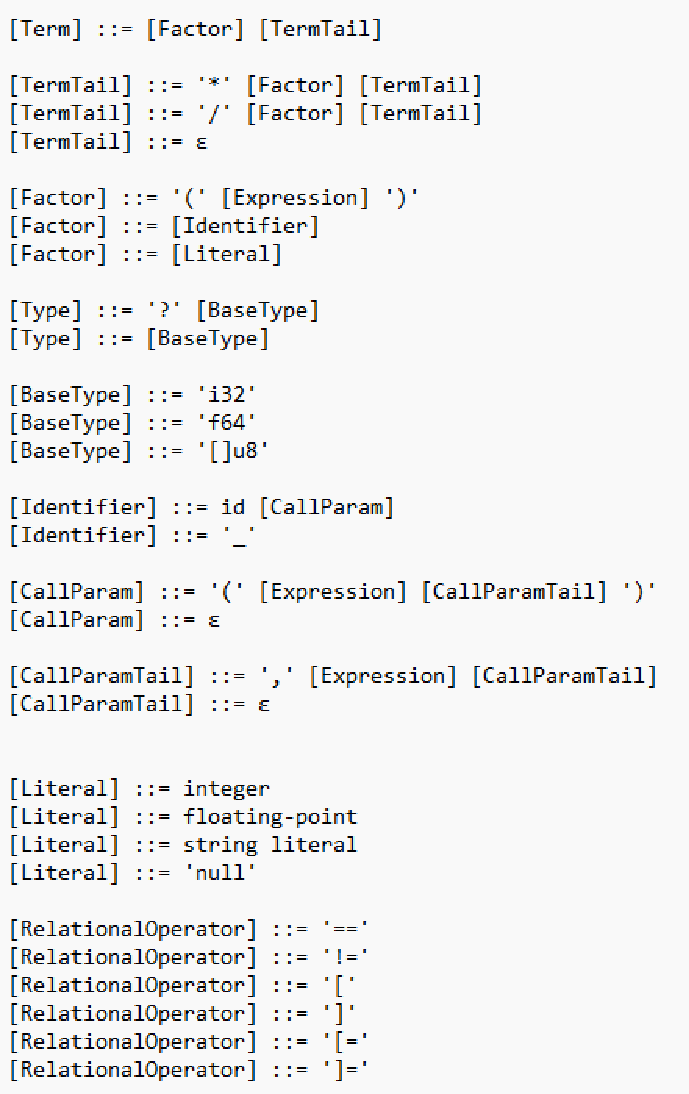
\includegraphics[width=0.7\linewidth]{Grammar2.pdf}
		\caption{Grammar 2}
		\label{table:png2pdf (2).pdf}
	\end{table}


	%\section{LL -- tabulka}
	%\begin{table}[!ht]
	%	\centering
	%	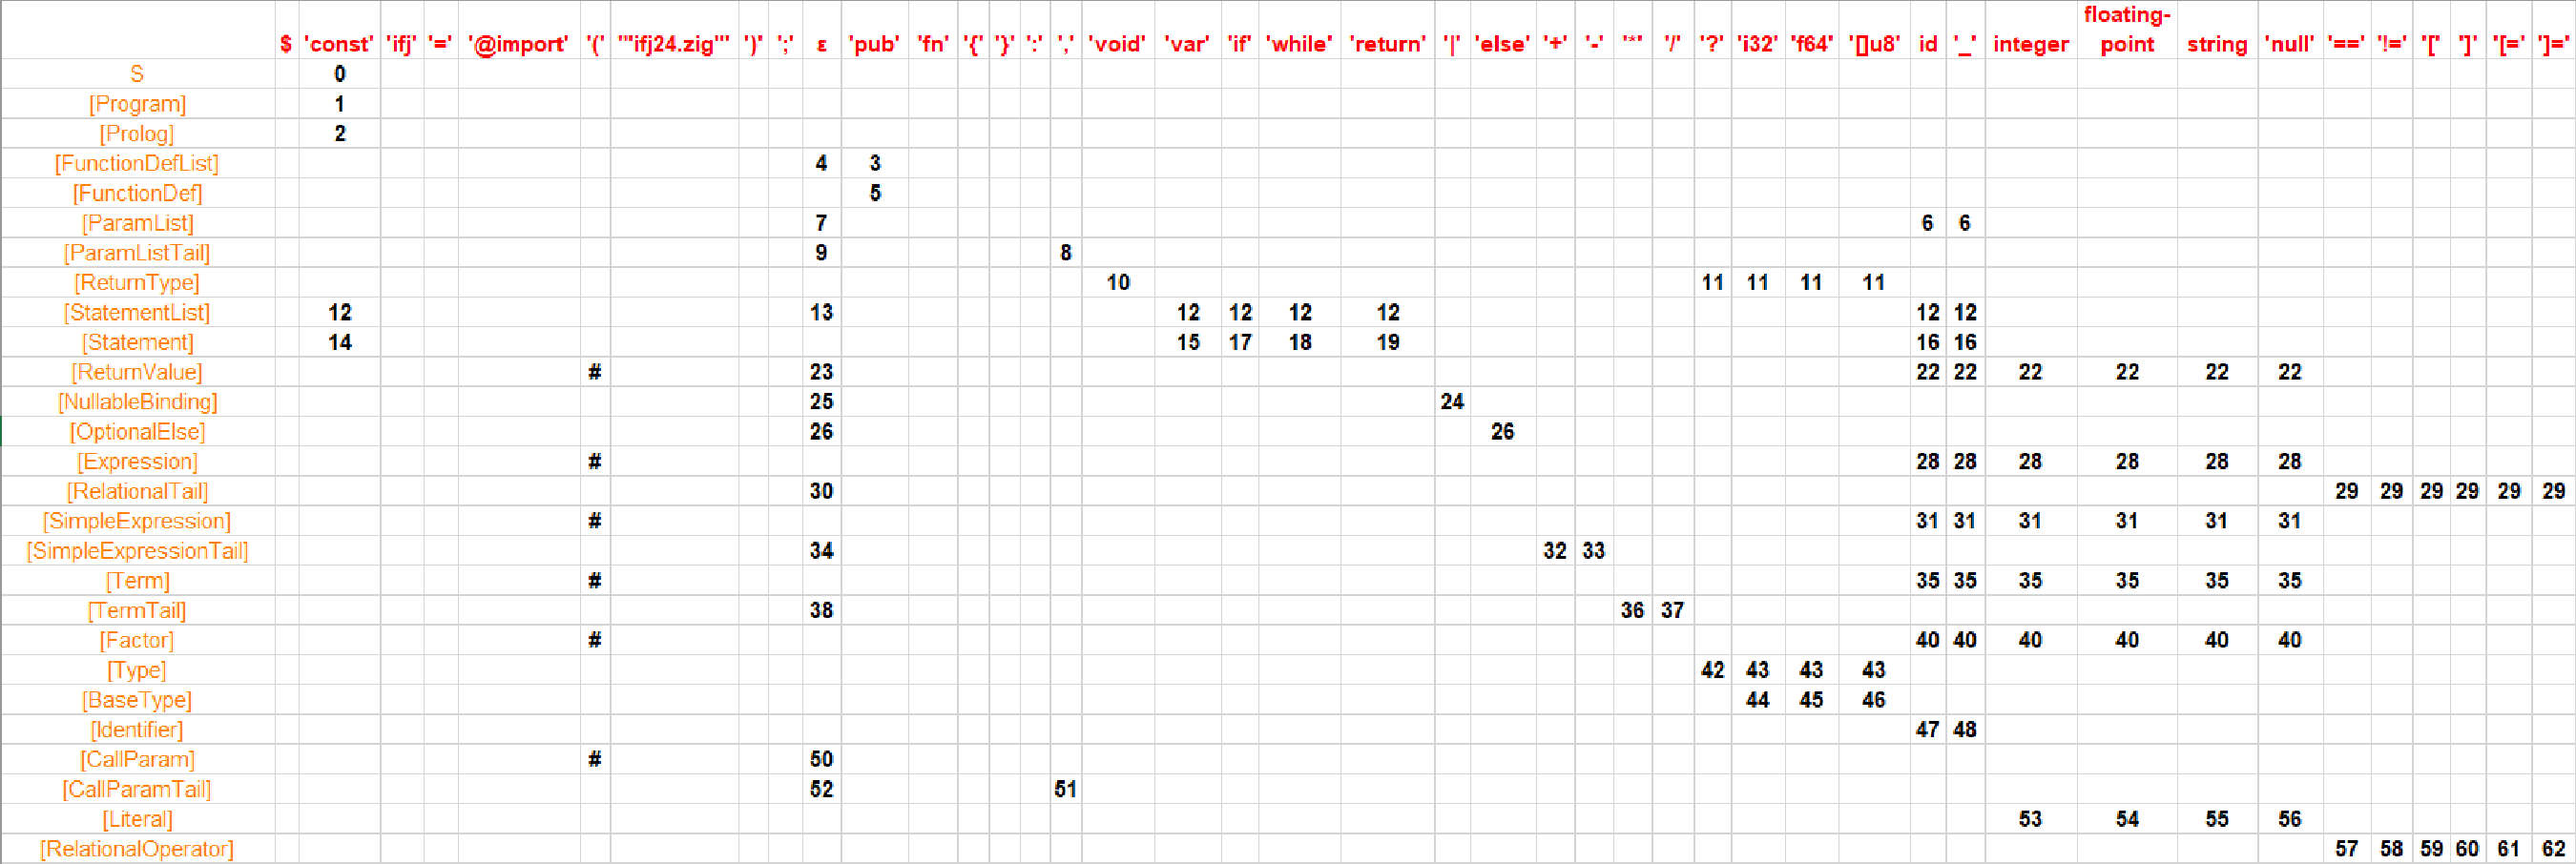
\includegraphics[width=1\linewidth]{inc/LL_table.pdf}
	%	\caption{LL -- tabulka použitá při syntaktické analýze}
	%	\label{table:ll_table}
	%\end{table}


	
	\begin{table}[!ht]
        \section{Precedence table}
		\centering
		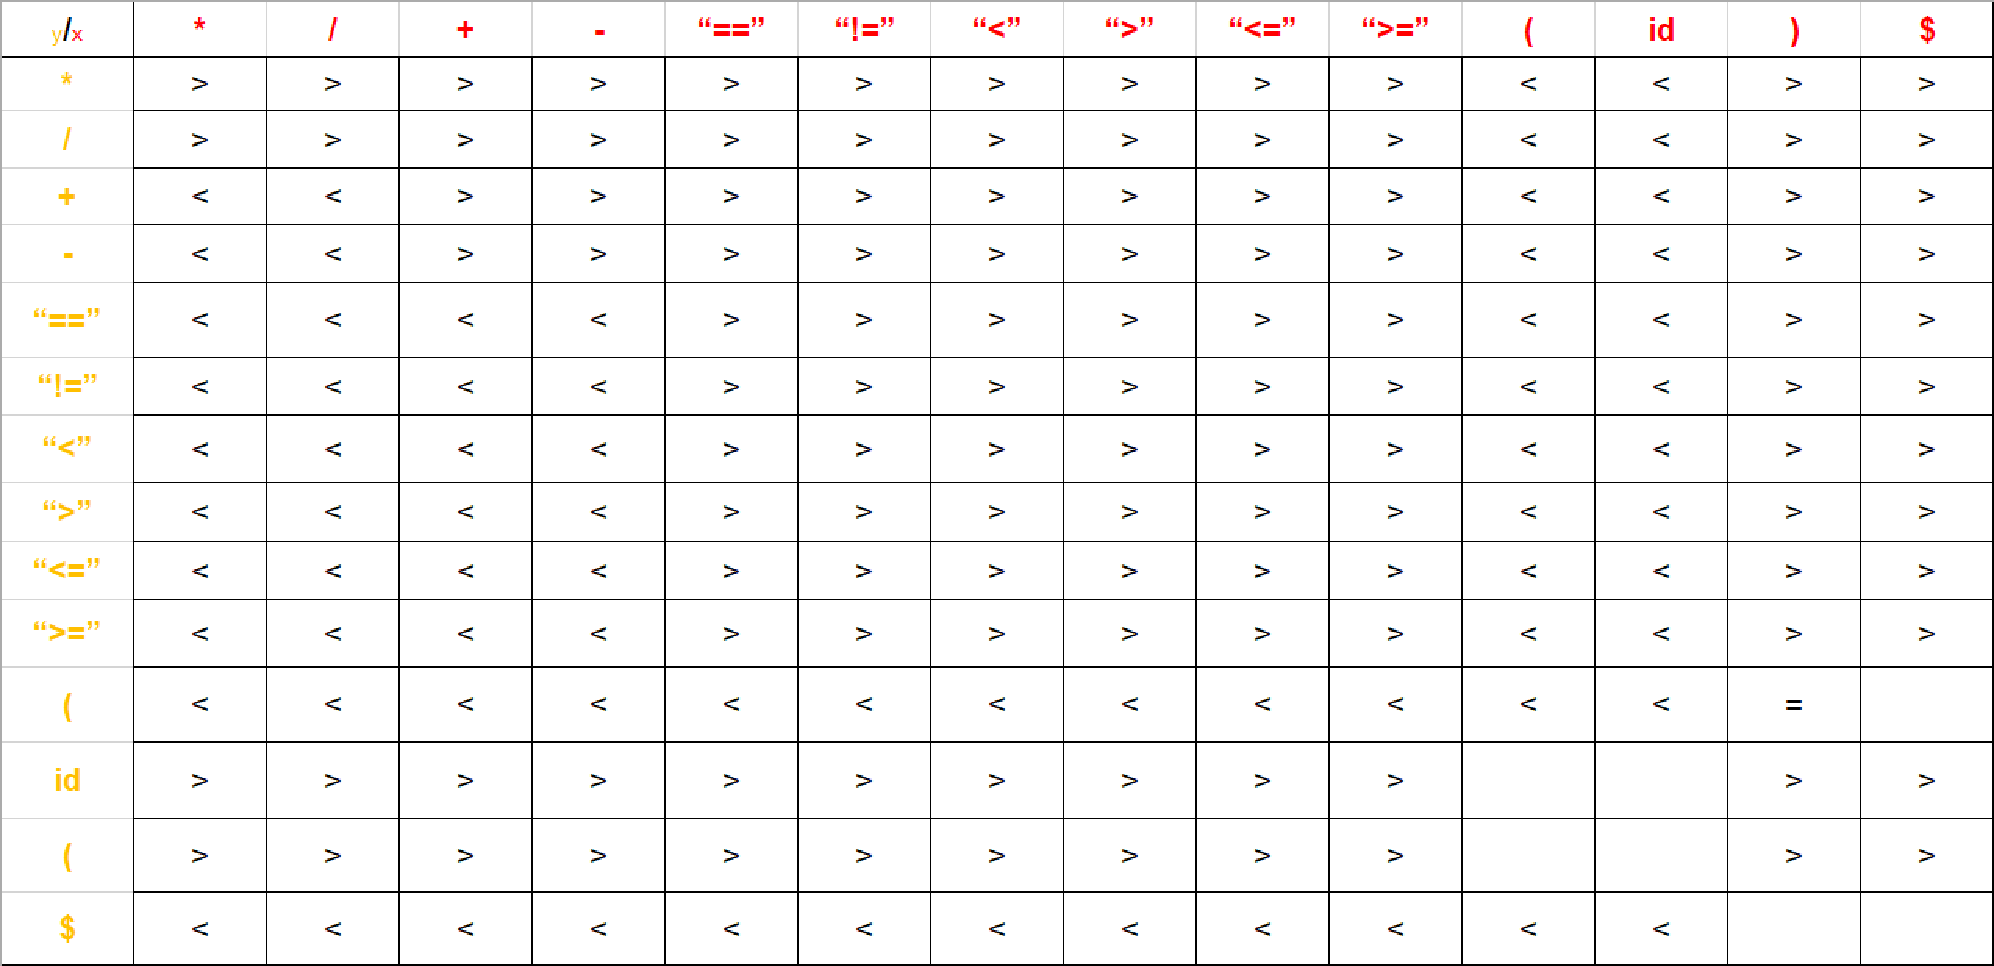
\includegraphics[width=0.7\linewidth]{Precedence table.pdf}
		\caption{Precedence table used in precedent syntactic analysis of expressions}
		\label{table:prec_table}
	\end{table}


\end{document}